\subsection{Evaluation}

After the completion of the modelling phase, the next step is to evaluate the results. The evaluation is split into 
the evaluation of the model itself followed by the evaluation of the overall process. 

\subsubsection{Gradient Boosting Evaluation}

In this section the Gradient Boosting algorithm will observed in more detail by the most common metrics. Additionally, it also
will be compared with the much simpler Classification Tree algorithm to highlight commonalities and different approaches between 
the two algorithms and create an all-encompassing picture for Gradient Boosting. 

The overall accuracy measured is around \(86\)\%. This result is already positive as the Gradient Boosting Algorithm outperforms 
the Classification Tree, which achieves an also respectable accuracy of \(80\)\%. However, the accuracy score can only be used as a
fundamental basis for evaluating the overall performance with many unknowns that need to be worked through.

The first step of a deeper analysis is to create a confusion matrix for all categories. The confusion matrix is an approach of 
visualizing the performance by clustering the the output. The \(x1\)-axis represents the predicted values for the classes 
while the \(x2\)-axis stands of actual (correct) values \cite[p.235]{Davis_2006}. The confusion matrix reveals four combinations of predicted 
and actual values (\ref{tbl:evaluation_confusion_matrix}). For Gradient Boosting the confusion matrix is displayed in table \ref{tbl:gb_confusion_matrix}.

\begin{table}[H]
  \centering
  \begin{tabular}{lrrrr}
    \toprule
    predicted & class 1         &  class 2          \\
    actual    &                 &                   \\
    \midrule
    class 1   &  true positive  &  false negative   \\
    class 2   &  false positive &  true negative    \\
    \bottomrule
    \end{tabular}
  \caption{Confusion matrix}%
  \label{tbl:evaluation_confusion_matrix}%
\end{table} 

\begin{table}[H]
  \centering
  \begin{tabular}{lrrrr}
    \toprule
    predicted & hiphop (1) & rock (2) & jazz (3) &   all \\
    actual &      &       &      &       \\
    \midrule
    hiohop &  438 &    68 &   19 &   525 \\
    rock   &   41 &  1307 &  122 &  1470 \\
    jazz   &   30 &   115 &  536 &   681 \\
    all    &  509 &  1490 &  677 &  2676 \\
    \bottomrule
    \end{tabular}
  \caption{Gradient Boosting Confusion Matrix}%
  \label{tbl:gb_confusion_matrix}%
\end{table} 

Visually, the highest misclassification takes place between classes \emph{jazz} and \emph{rock} while the lowest missclassification occurs
between \emph{hiphop} and \emph{jazz}. This result however has little significance, since the number of \emph{rock} tracks, with a total of over 
\(1400\), is significantly larger than the amount of both \emph{hiphop} and \emph{jazz} tracks. An evaluation based on absolute numbers would lead to 
misleading results partly due to the imbalance of the dataset. 

A better approach is to look at the following metrics which can be derived form the confusion matrix for every category \cite[p.235]{Davis_2006} \cite[p.862]{fawcett2006introduction}(\ref{tbl:gb_classification_Report}). 

\begin{equation*}
  \begin{aligned}
    precision &= \;\frac{true\:positive}{true\:positive\;+\;false\:positive}
    \\
    recall &= \;\frac{true\:positive}{true\:positive\;+\;false\:negative}
    \\
    f1-score &= \;2\;*\;\frac{precision\;*\;recall}{precision\;+\;recall}
  \end{aligned}
\end{equation*}

\begin{table}[H]
  \centering
  \begin{tabular}{lllll}
    \toprule
    classes & precision & recall & f1-score & support \\
    \midrule
     hiphop &      0.86 &   0.83 &     0.85 &     525 \\
       rock &      0.88 &   0.89 &     0.88 &    1470 \\
       jazz &      0.84 &   0.79 &     0.79 &     681 \\
    \bottomrule
    \end{tabular}
  \caption{Gradient Boosting Classification Report}%
  \label{tbl:gb_classification_Report}%
\end{table} 

Precision and recall are both performance metrics with different objectives. While precision is a measure of how many of the 
predicted elements for a class were correct, recall measures how many elements of a category were detected. It can be observed that 
the precision is high across all categories with \emph{rock} being classified best with \(12\)\% false-positive predictions while 
the false-positive rate for \emph{jazz} was worst with over \(21\)\%. Interestingly the results for recall are very similar with the model 
performing best for the category \emph{rock} with an recall of \(0.89\) and again worst for \emph{jazz} with \(0.79\). For both metrics \emph{Hiphop} is in
between of both extremes at around \(0.85\). 

The f1-score is a combination out of precision and recall and an attempt of capturing both metrics in a single value. Therefore,
the results are not surpising. \emph{Jazz} performed worst with only \(0.79\) while \emph{rock} was classified best with \(0.88\) according to the 
f1-score. 

In conclusion all scores can be evaluated as positive outputs without any negative and unexplainable abnormalities. Also, in comparison 
to decision trees, a clear improvement of the results can be seen. The reason that \emph{jazz} is ranked worst while \emph{rock} reaches the 
highest values may be due to several reasons. One possible explanation can be found by reviewing the findings from the data 
understanding chapter. It is recognizable that the value-ranges for the features of \emph{jazz} were significantly more distributed 
than for both \emph{rock} and \emph{hiphop} and often without any high points. In addition, the value ranges of \emph{rock} were often different from 
those of hip-hop and jazz, which simplifies the respective classification. 

Another measure to evaluate a models performance is to plot its \ac{ROC}. The \ac{ROC} is a plot of the true-positive
rate for the \(x1\)-axis and the false-positive rate on the \(x2\)-axis for every possible threshold. The benefit of \ac{ROC} is that it plots the 
misclassification for every threshold while other metrics rely on a single threshold. A model whose results are close to the diagonal classifies data worse than a 
model whose curve is as close as possible to the point \((0/1)\) in the coordinate system. This performance is often measured by means of 
the \ac{AUC}, which is directly derived from the \ac{ROC}. With help of the \ac{AUC} comparability between models is possible \cite[p.862f]{fawcett2006introduction} \cite{scikit-roc_and_auc}. 
The \ac{ROC} and \ac{AUC} for the project are shown in figure \ref{fig:roc_and_auc_for_gb_and_dt}. 

%The categories are 
%replaced by numbers from \(0\) tot \(2\) which label the classes \emph{hiphop}, \emph{rock} and \emph{jazz} in the following order. 

  \begin{figure}[H]
    \centering
    \subfloat[\centering Gradient Boosting]{{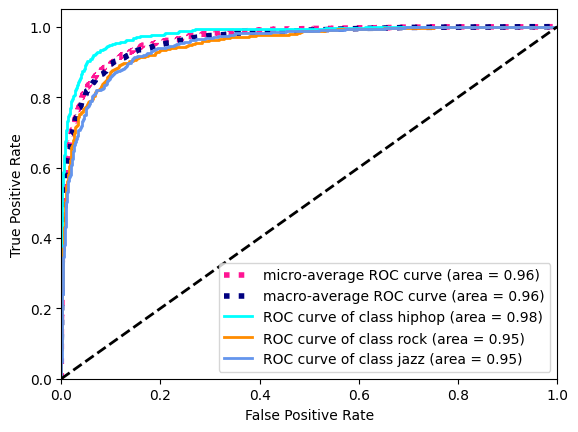
\includegraphics[width=6cm]{gb_roc_and_auc.png} }}%
    \qquad
    \subfloat[\centering Classification Tree]{{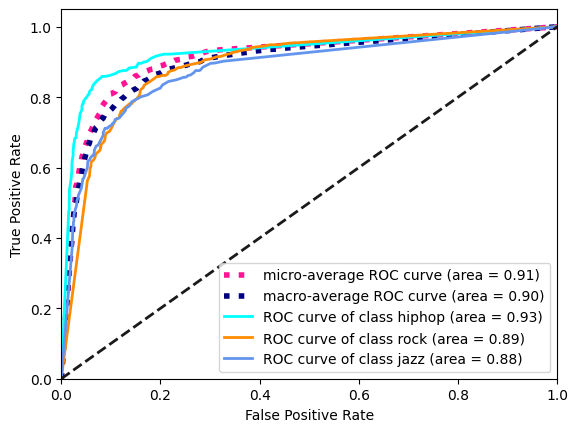
\includegraphics[width=6cm]{dt_roc_and_auc.png} }}%
    \caption{Comparison of ROC and AUC}%
    \label{fig:roc_and_auc_for_gb_and_dt}%
\end{figure}

The following matrix shows that the model works well for all classes. Both \ac{ROC} and the associated \ac{AUC} are convincing 
in all cases. Interesting is the fact that \emph{rock} has the worst \ac{AUC} while being classified best according to the previous metrics.
\emph{Hiphop}, on the other hand, has the significantly best \ac{AUC} followed by \emph{jazz}. An explanation for this result is complicated, with a 
possible reason again being the imbalance of the dataset. The model is focussed classifing \emph{rock} correctly as it constitutes to a large part of the 
dataset. Therefore, the optimum for both \emph{jazz} and \emph{hiphop} are exchanged for an overall optimum. It should be noted that a well-founded explanation would 
explanation would require a more in-depth analysis. Regardless, the result is worth including in the analysis and leaves room for 
further research.   

In addition, a very different evaluation can be performed. It is also interesting to take a closer look on the input data with help of 
the so-called feature importance. The feature importance is a measure of how much impact a feature had for the classification of the 
dataset and is presented in the following figure \ref{fig:feature_inportance_for_gb_and_dt} for both Gradient Boosting and the Classification Tree algorithm
\cite{scikit-learn_feature_importance}. 

\begin{figure}[H]
  \centering
  \subfloat[\centering Gradient Boosting]{{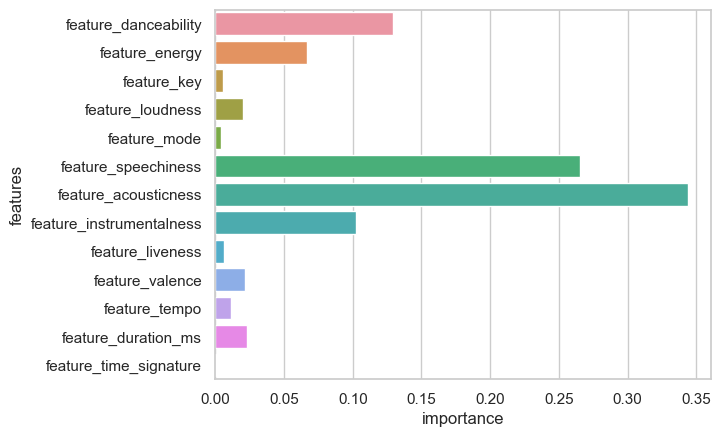
\includegraphics[width=6cm]{gb_feature_importance.png} }}%
  \qquad
  \subfloat[\centering Classification Tree]{{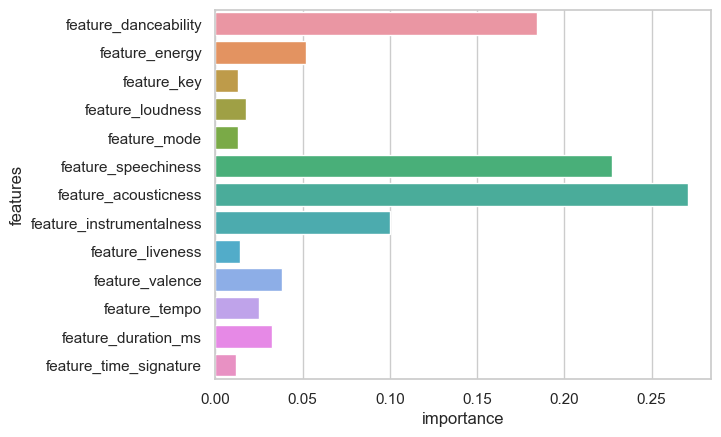
\includegraphics[width=6cm]{dt_feature_importance.png} }}%
  \caption{Comparison of Feature Importance}%
  \label{fig:feature_inportance_for_gb_and_dt}%
\end{figure}

It is clearly visible that both Gradient Boosting and Decision Trees relied on similiar features to similar extends for the classification task with 
minor differences for features such as \emph{danceability}. Noticeable is that Gradient Boosting is heavily focused on only a few features 
while the Classification Tree makes more use out of features like \emph{duration}, \emph{valence} and \emph{mode}. One possibility for the difference in weighting  
could be the overall construction of the algorithms. Gradient Boosting consists out of multiple weak learners while the Classification Tree
algorithm froms a widely branched and deep tree. For feature importance, an analogy can again be made with data understanding and music theory. 
The features that theoretically distinguish the genres from another play the most important role for the modeling while musical standards and 
more subjective featues only play a subordinate role. This result is positive both for theory and the machine learning model as it states 
that music theory can be confirmed by real-world examples while giving credibility and plausibility to the model.

\subsubsection{Process Evaluation}

The evaluation of the overall process is complicated as there are many unknowns starting with the dataset itself. The data used is preprocessed by 
Spotify without detailed definition and theoretical basis. The features are furthermore heavily subjective, which adds another layer of 
complexity. Also the data collection is non-trivial and error-prone. Both the collection process and the collection approach 
would have to be revised for a productive use case. On the other hand, the data quality is decent with high correlation to the music 
theory. In addition, the dataset convinces with its uniqueness and novelty.

The model in combination with preprocessing and evaluation also leaves room for further research. The use of only two very 
similar machine learning algorithms allows no comparison to completely differnt approaches based on other algorithms and concepts. 
It can therefore not be ruled out that even better results can be achieved. The pre-processing is intensive with many constallations 
tested. A possible improvement would be to apply the hyperparametric optimization not only on the standardized data but on all 
approaches to ensure an overall best result. In addition, there are further hyperparameter constellations which were not tested.
The evaluation may also have reached incorrect conclusions and assumptions for a variety of reasons. 

The overall highest risk is the fact that all participants of the group are not familiar with machine learning and lack 
experience. For this reason, the result can be considered promising, as both algorithms provide good overall results.

%
%Daten:
%s
%- vorprozessiert von Spotify
%- oft auch interpretation und subjektiv
%- keine eindeutige Definition, was Aussagekraft schwierig macht
%- Datensammlung -> Ungenau, fehleranfällig, jedoch gute und sehr interessante Datenbasis
%
%Modelle:
%
%- Korrektes Modell gewählt? -> kein Vergleich 
%
%Vorprozessierung, Klassifikation und Auswertung: 
%
%- hyperparameter nur auf standardized 
%- Mehr optionen zu hyperparameter
%- Evaluation und Schlüsse korrekt? -> Daten vielleicht nicht aussagekräftig
%- Allgemein viel selbstgeschriebenes Coding -> fehleranfällig, da neu in Materie